\documentclass[14pt,a4paper]{extarticle}

% Язык РУ

% Шрифт (Times New Roman)
\usepackage{fontspec}
\setmainfont{Times New Roman}
\setmonofont{Times New Roman}

\usepackage{listings}
\newfontfamily\codefont{Courier New}
\lstset{
    basicstyle=\fontsize{12pt}{12pt}\selectfont\codefont,
    backgroundcolor=\color{white},
    keywordstyle=\color{black},
    stringstyle=\color{black},
    commentstyle=\color{black},
    identifierstyle=\color{black},
    numbers=none,
    showstringspaces=false,
    breaklines=true,
    frame=none
}

\usepackage{polyglossia}
\setdefaultlanguage{russian}

% Межстрочный интервал 1.5
\usepackage{setspace}
\onehalfspacing
\newfontfamily\cyrillicfont{Times New Roman}

% Красная строка
\setlength{\parindent}{12.5mm}
\setlength{\parskip}{0pt}

% Выравнивание по ширине (по умолчанию есть, но фиксируем)
\usepackage{ragged2e}
\justifying

% Нумерация страниц
\usepackage{fancyhdr}
\pagestyle{fancy}
\fancyhf{} % очищаем колонтитулы
\fancyfoot[C]{\thepage} % номер страницы по центру снизу
\renewcommand{\headrulewidth}{0pt} % убираем линию сверху

% Заголовки с новой страницы
\usepackage{titlesec}
\renewcommand{\thesection}{\arabic{section}.}
\titleformat{\section}{\normalsize\bfseries}{\thesection}{0.5em}{}
\titlespacing*{\section}{\parindent}{0pt}{0pt}

\let\oldsection\section
\renewcommand{\section}{\clearpage\oldsection}

\newcommand{\structsection}[1]{
  \addcontentsline{toc}{section}{\MakeUppercase{#1}}
  \clearpage
  \noindent{\centering\textbf{\MakeUppercase{#1}}\par}
}
\newcommand{\fakeSection}[2][]{}

\usepackage{csvsimple}
\usepackage{tabularx}
\usepackage{float}
\usepackage{array}



\usepackage{wrapfig}

\usepackage{tocloft}
\renewcommand{\cfttoctitlefont}{\hfill\bfseries\MakeUppercase}
\renewcommand{\cftaftertoctitle}{\hfill}

% Убираем полужирный шрифт у разделов в содержании
\renewcommand{\cftsecfont}{\normalfont}
\renewcommand{\cftsecpagefont}{\normalfont}

% Поля
\usepackage[
    left=30mm,
    right=15mm,
    top=20mm,
    bottom=20mm
]{geometry}


\usepackage{indentfirst}

\usepackage{pdfpages}
\usepackage{microtype}
\emergencystretch=2em
\righthyphenmin=2
\sloppy

\usepackage{array}

\usepackage{caption}
\captionsetup[table]{justification=raggedright,singlelinecheck=false}
\renewcommand{\tablename}{Таблица}
\captionsetup[table]{labelsep=endash}
\usepackage{tabularx}
\usepackage{array}
\newcolumntype{C}{>{\centering\arraybackslash}p{2cm}}
\usepackage{longtable}
\usepackage{ltablex}
\keepXColumns

\usepackage{enumitem}

\newlist{myenum}{enumerate}{1}
\setlist[myenum]{
    label=\arabic*) ,
    leftmargin=\parindent,
    labelwidth=!,
    labelsep=0.1cm,
    align=left,
    itemsep=1em,
    parsep=0pt
}

\newlist{myitem}{itemize}{1}
\setlist[myitem]{
    label=\textbullet,
    leftmargin=\parindent,
    labelwidth=!,
    labelsep=0.1cm,
    align=left,
    itemsep=1em,
    parsep=0pt
}

\usepackage{amsmath}
\usepackage{amssymb}
\usepackage{amsthm}
\usepackage{mathtools}

\usepackage{indentfirst}

\makeatletter
% Теорема (с аргументом)
\newenvironment{my_theorem}[1][Теорема]
{\par\indent\noindent{#1.} \upshape}
{\par}

% Утверждение (с аргументом)
\newenvironment{my_statement}[1][Утверждение]
{\par\indent\noindent{#1.} \normalfont}
{\par}
\makeatother
\setlength{\parindent}{1.5cm}

% Пример (без аргумента)
\newenvironment{my_example}
{\par\indent\noindent{Пример.} \upshape}
{\par}

% Доказательство (с символом в конце)
\newenvironment{my_proof}
{\par\indent\noindent{Доказательство.} \upshape}
{\par\hfill $\square$}

\makeatother

\usepackage{silence}

\WarningFilter{biblatex-gost}{You set maxbibnames}

\usepackage{csquotes}
\usepackage[
backend=biber,
style=gost-numeric,
sorting=none,
maxbibnames=99,
maxcitenames=99
]{biblatex}
\DefineBibliographyStrings{russian}{
  urlseen = {дата обращения}
}
\addbibresource{article_main.bib}


\defbibenvironment{bibliography}
  {\begin{spacing}{1.5}
   \list
     {\printfield{labelnumber})}
     {\setlength{\leftmargin}{0cm}
      \setlength{\itemindent}{2.3cm}
      \setlength{\labelsep}{0.5cm}
      \setlength{\itemsep}{0.5em}
      \setlength{\parsep}{0pt}
     }}
  {\endlist
   \end{spacing}}
  {\item}

\usepackage{caption}
\DeclareCaptionLabelFormat{gostfigure}{Рисунок #2}
\captionsetup[figure]{labelformat=gostfigure,labelsep=endash,justification=centering}



%%% СПИСКИ (ENUMITEM) %%%
\usepackage{enumitem}
% Маркированный список (тире, отступ 1.25)
% Маркированный список: тире на 1.25см, перенос — от края страницы
\setlist[itemize,1]{
    label=—, 
    leftmargin=0pt,       % Весь блок текста прижат к левому краю (0см)
    labelindent=\parindent,   % Само тире начинается на отметке 1.25см
    labelsep=0.5em,       % Расстояние от тире до текста
    itemindent=*,         % Рассчитывает отступ первой строки, чтобы метка встала на 1.25см
    nosep,
    font=\normalfont
}
\setlist[itemize,2]{label=—, leftmargin=0pt, itemindent=2.5cm, labelsep=0.5em, nosep}

% Нумерованный список: цифра начинается на 1.25см, перенос — от края страницы
\setlist[enumerate,1]{
    label=\arabic*), 
    leftmargin=0pt,       % Весь блок текста прижат к левому краю (0см)
    labelindent=\parindent,   % Сама цифра (номер) начинается на отметке 1.25см
    labelsep=0.5em,       % Расстояние от скобки до текста
    itemindent=*,         % Автоматически рассчитывает отступ первой строки, чтобы цифра встала на 1.25см
    nosep
}

% Второй уровень маркированного списка
\setlist[itemize,2]{
    label=—, 
    leftmargin=0pt,       % Перенос текста к 0см
    labelindent=2\parindent,    % Отступ тире 2.5см от края страницы
    labelsep=0.5em, 
    itemindent=*, 
    nosep
}

\setlist[enumerate,2]{
    label=\arabic{enumi}.\arabic*), % Использовать enumi вместо maxleveli
    leftmargin=0pt,        
    labelindent=2\parindent,    
    labelsep=0.5em,        
    itemindent=*,          
    nosep
}


\begin{document}

% 1. Титульный лист (внешний PDF)
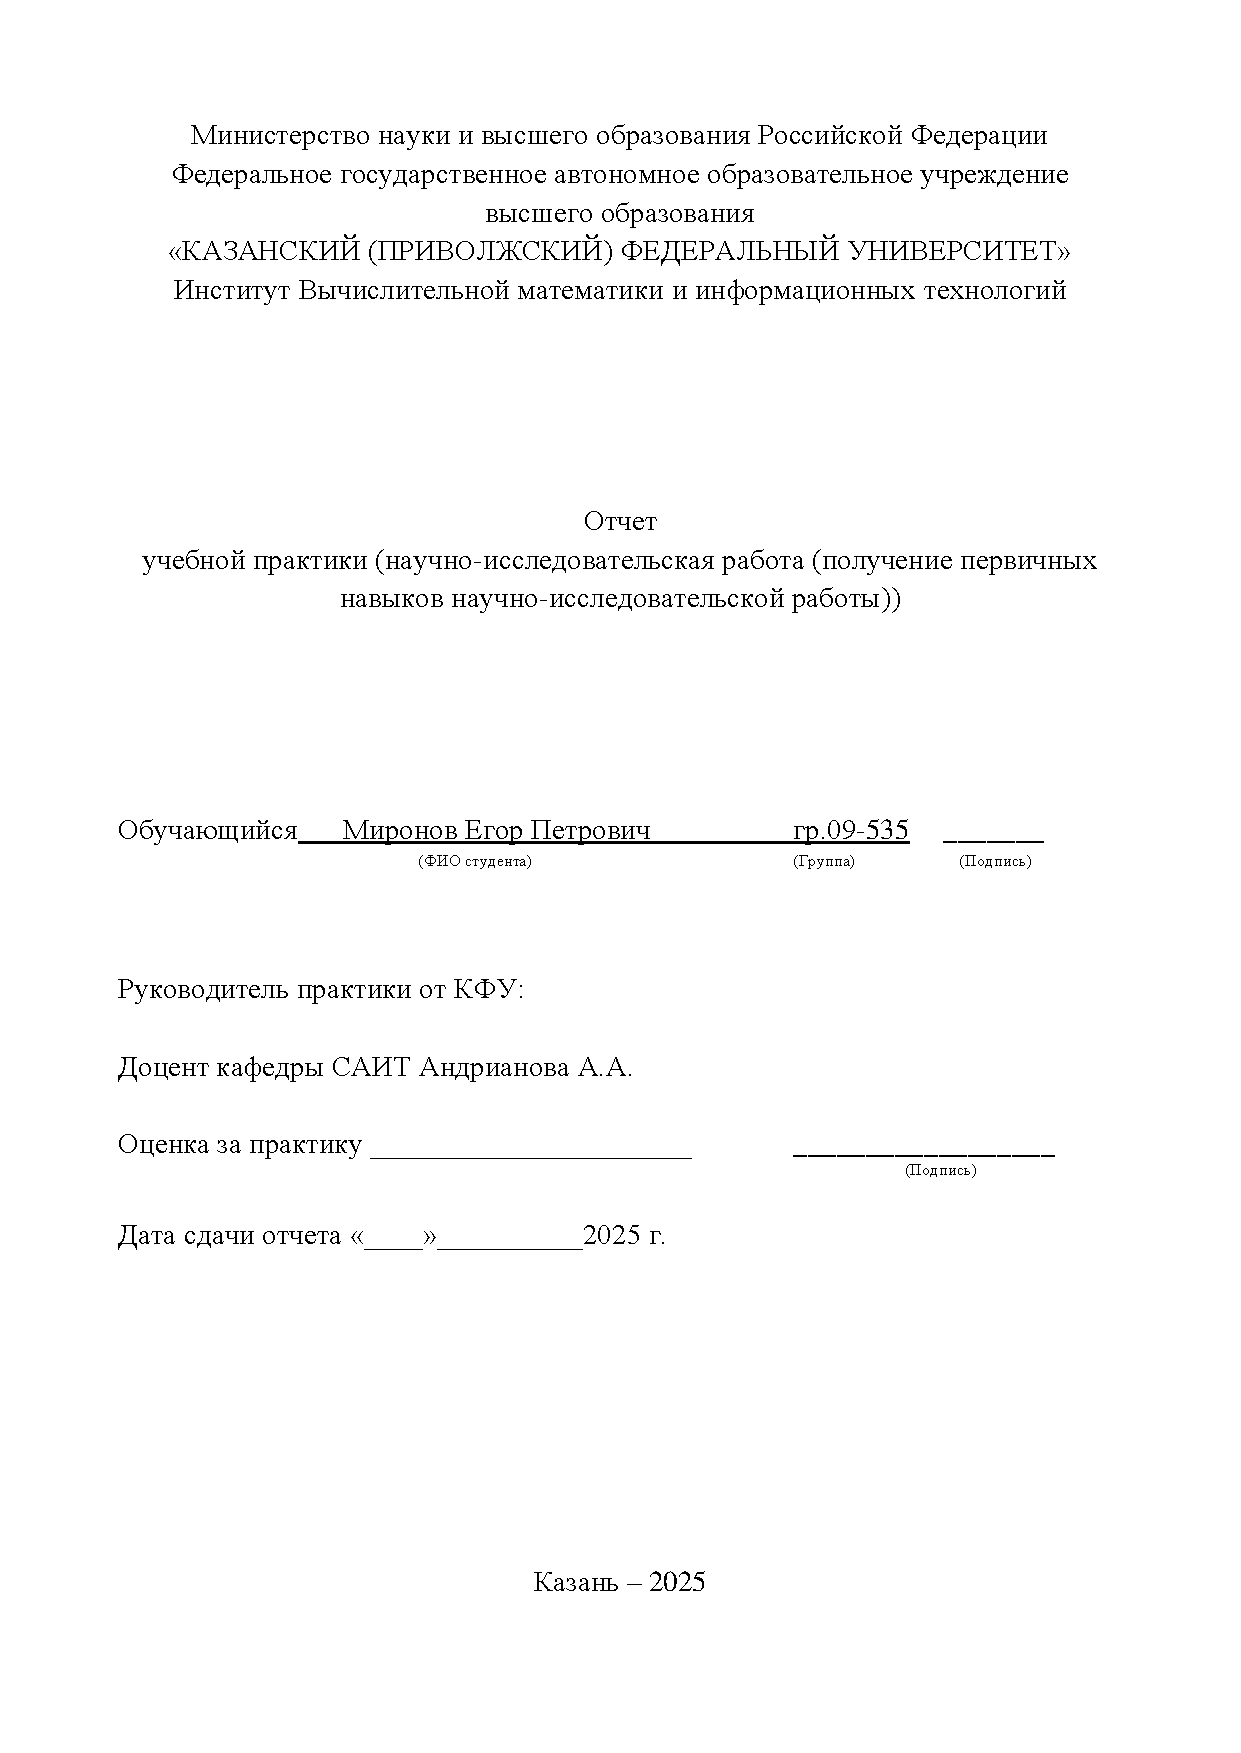
\includepdf[pages=1]{титул.pdf}
\setcounter{page}{2}

% 2. Содержание
\clearpage
\tableofcontents
\newpage

% 3. Введение
\structsection{Введение}

Учебная практика (научно-исследовательская работа (получение первичных навыков научно-исследовательской работы)) проходила на кафедре системного анализа и информационных технологий Института вычислительной математики и информационных технологий КФУ с 01 сентября 2025 года по 30 декабря 2025 года.

Целью практики является выполнение начальных этапов научно-исследовательской работы над темой магистерской диссертации, включающей выбор темы и изучение методов решения выбранной задачи на текущий момент.

Выбранная задача посвящена исследованию и анализу подходов к автоматизированному распознаванию и классификации транзакций на основе анализа изображений. В рамках работы рассматриваются изображения финансовых документов, включая чеки, квитанции, снимки экрана финансовых операций и иные визуальные источники, содержащие информацию о финансовых транзакциях. 

Основное внимание уделяется анализу существующих подходов к обработке таких данных и формированию представления о возможных направлениях дальнейшего исследования.

\fakeSection[opt]{text}

% 4. Основная часть
\structsection{Основная часть}

В условиях активного развития цифровых финансовых сервисов существенно увеличивается объём транзакционных данных, используемых как частными пользователями, так и организациями~\cite{shendo2024}. Значительная часть информации о финансовых операциях представляется в виде визуальных документов, включая чеки, квитанции, снимки операций из мобильных банковских приложений, отчёты и иные графические форматы. Такие данные широко используются в системах учёта личных финансов, бухгалтерских приложениях и аналитических сервисах. Наиболее распространенные типы финансовых документов и их особенности представлены в таблице ~\ref{tab:finance_docs_type}.

\begin{tabularx}{\textwidth}{|X|X|X|X|}
    \caption{Типы финансовых документов и их особенности.} \label{tab:finance_docs_type} \\ 

    \hline 
    Тип документа & Пример источника & Характерные особенности & Проблемы автоматизированной обработки \\ \hline
    \endfirsthead

    \caption{Типы финансовых документов и их особенности.} \\ 
    \hline Тип документа & Пример источника & Характерные особенности & Проблемы автоматизированной обработки \\ \hline 
    \endhead
    Кассовый чек & Розничные магазины, супермаркеты & Небольшой размер текста, термопечать, нестабильное качество изображения, наличие QR-кодов и сокращений & Шумы, низкая контрастность, смазанность символов, частичная потеря текста, ошибки OCR \\ \hline Электронный чек & Интернет-магазины, маркетплейсы & PDF-формат или скриншот, наличие гиперссылок и цифровых идентификаторов & Различие структур документов, наличие служебных элементов интерфейса \\ \hline Квитанция об оплате & Коммунальные услуги, государственные сервисы & Структурное представление данных, фиксированные поля и реквизиты & Различия шаблонов, неоднородное расположение полей, сложность выделения ключевых атрибутов \\ \hline Банковская выписка & Интернет-банкинг, PDF-отчёты & Табличная структура, большое количество транзакций, многострочные записи & Сложность сегментации таблиц, переносы строк, неоднозначность категорий операций \\ \hline Скриншот транзакции & Мобильные банковские приложения & Наличие элементов пользовательского интерфейса, иконок, уведомлений, динамических блоков & Избыточные визуальные элементы, неоднородный фон, адаптивная вёрстка интерфейсов \\ \hline Фотография бумажного документа & Камера мобильного устройства & Перспективные искажения, неравномерное освещение, тени & Геометрические деформации, шумы, потеря читаемости текста \\ \hline Документы с рукописными элементами & Квитанции с подписями и пометками & Комбинация печатного и рукописного текста & Низкая точность распознавания рукописных символов, неоднородность почерка \\ \hline \end{tabularx}


Несмотря на высокий уровень цифровизации~\cite{yakovleva2023}, автоматизированная обработка изображений финансовых документов остаётся сложной задачей. Финансовые документы отличаются высокой вариативностью структуры, форматов и качества изображений. Документы могут быть получены с различных устройств, содержать шумы, искажения, частично утраченные данные, а также различаться по языку, валюте и способу представления информации. Эти особенности существенно осложняют процесс автоматического анализа и требуют применения интеллектуальных методов обработки.

Существующие решения в области автоматизации финансового учёта, как правило, ориентированы на работу с ограниченным набором источников данных или поддерживают только отдельные форматы документов. Многие приложения корректно функционируют лишь при интеграции с конкретными банками или сервисами, что снижает универсальность подобных систем. При этом задача обработки изображений транзакций, полученных из произвольных источников, зачастую остаётся нерешённой или требует ручного вмешательства пользователя.

Таким образом, задача разработки и исследования универсальных подходов к автоматизированному распознаванию и анализу изображений финансовых документов является актуальной. Решение данной задачи позволит повысить уровень автоматизации финансовых сервисов, снизить влияние человеческого фактора и создать основу для дальнейшего интеллектуального анализа транзакционной информации.


Целью исследования является анализ и обоснование подходов к созданию автоматизированной системы распознавания и классификации транзакций на основе анализа изображений финансовых документов.

Для достижения поставленной цели в рамках работы предполагается решение следующих задач:

\begin{enumerate} 
  
\item анализ предметной области и типов транзакционных документов:

\begin{enumerate}

\item изучение существующих методов обработки,

\item обзор и анализ подходов к классификации транзакций,

\item исследование возможностей мультимодальных методов.

\end{enumerate}

\item формирование концепции автоматизированной системы.

\end{enumerate}

Сформулированная задача автоматизированного распознавания и классификации транзакций на основе изображений финансовых документов является комплексной и включает несколько взаимосвязанных этапов обработки данных. Эффективное решение данной задачи невозможно без использования современных методов компьютерного зрения и интеллектуального анализа данных~\cite{panteleeva2025}.

Для обоснованного выбора направления дальнейшего исследования и формирования концепции автоматизированной системы необходимо рассмотреть существующие методы и подходы, применяемые для обработки изображений документов и анализа содержащейся в них информации, а именно:

\begin{enumerate} 
\item современные методы оптического распознавания текста,
\item принципы извлечения структурированной информации,
\item методы классификации финансовых данных,
\item инновационные мультимодальные подходы.
\end{enumerate}

\section{Методы оптического распознавания текста}

Оптическое распознавание текста (OCR) является одной из ключевых технологий для автоматизированной обработки изображений~\cite{vorozhtsova2019}. OCR позволяет преобразовывать графические представления текста в машинно-читаемый формат, что является необходимым этапом для последующей структуризации и классификации транзакций.

По обыкновению процесс оптического распознования текста задается в виде следующей формулы: $f : I \rightarrow T$. Функция $f$ описывает процесс преобразования визуального представления документа в текстовое описание, где $I$ - изображение документа, $T$ - распознанная текстовая последовательность.

Существующие методы OCR можно условно разделить на классические и современные нейросетевые подходы~\cite{davletov2023}. К классическим относятся алгоритмы на основе сегментации символов и шаблонного сопоставления, которые хорошо работают с чётким текстом стандартных шрифтов, но показывают ограниченную эффективность на изображениях с шумами, искажениями или нестандартными форматами документов. Современные нейросетевые подходы используют сверточные нейронные сети (CNN), рекуррентные сети (RNN) и трансформеры для распознавания текста в условиях вариативных и сложных визуальных данных. $\mathcal{L}_{CTC} = - \log \sum_{\pi \in \mathcal{B}^{-1}(y)} P(\pi \mid \mathbf{x})$.

В сверточных сетях извлечение признаков выполняется посредством операции свёртки:
\begin{gather*}
(I*K)(x,y)=
\sum_m \sum_n I(m,n)K(x-m,y-n).
\label{eq:convolution}
\end{gather*}

Полученные признаки далее преобразуются в вероятностное распределение классов символов с использованием функции softmax $P(y_i)=
\frac{e^{z_i}} {\sum_j e^{z_j}}$, где $z_i$ представляет значение логита для класса $i$.

Для обучения OCR-моделей применяется функция потерь cross-entropy:
\begin{gather*}
L(\theta)=
-\sum_{i=1}^{N}
\Big(
y_i \log \hat{y}_i
+
(1-y_i)\log(1-\hat{y}_i)
\Big).
\label{eq:loss}
\end{gather*}

Такие модели обладают высокой устойчивостью к искажениям, разным шрифтам и сложной структуре документа~\cite{nestorov2020}. Также стоит отметить, что в современных системах, основанных на искусственном интеллекте, OCR ищет текст $T$, который максимизирует вероятность правильного распознавания при заданном изображении $I$. Таким образом современные OCR-системы решают задачу поиска наиболее вероятной текстовой последовательности $\hat{T}$ для входного изображения $I$, согласно формуле
$\hat{T} = \arg\max_T P(T|I)$.

При обработке финансовых документов OCR сталкивается с рядом специфических проблем: низкое качество сканов или фотографий, различие в форматах чеков и квитанций, наличие штрих- и QR-кодов, а также смешение текста и графических элементов. 

\begin{my_statement}
Предварительная обработка изображения позволяет уменьшить
количество ошибок сегментации символов
и повысить качество последующего OCR-распознавания.
\end{my_statement}

\begin{my_proof}
Рассмотрим изображение документа,
представленное функцией интенсивности $I : \Omega \rightarrow \mathbb{R}$, где $\Omega$ - множество пикселей изображения.

На исходном изображении могут присутствовать шум,
неравномерное освещение,
артефакты сжатия и слабый контраст текста.
Подобные искажения усложняют процесс выделения символов
и приводят к ошибкам сегментации.

Для повышения качества изображения
применяется этап бинаризации,
в рамках которого изображение преобразуется
в двоичное представление:

\begin{equation*}
B(x,y)=
\begin{cases}
1, & I_f(x,y) \geq \tau, \\
0, & I_f(x,y) < \tau,
\end{cases}.    
\end{equation*}

В результате бинаризации
формируется изображение,
содержащее только два класса пикселей:
фон и текстовые области.

Для оценки качества сегментации
можно рассмотреть отношение сигнал/шум $SNR=\frac{\mu_s}{\sigma_n}$.

После бинаризации и предварительного сглаживания
значение $SNR$ возрастает,
так как уменьшается влияние высокочастотного шума
и усиливается контраст между текстом и фоном.

Дополнительно уменьшается количество ложных границ,
возникающих при детектировании контуров символов.
Это упрощает процесс локализации текстовых областей
и снижает вероятность ошибочного разделения символов.

Пусть множество корректно сегментированных символов
обозначается через $C$,
а множество ошибок сегментации через $E$.
Тогда качество сегментации можно оценить по формуле 
$Q=\frac{|C|}{|C|+|E|}.$

После применения предварительной обработки
значение $|E|$ уменьшается,
а показатель $Q$ возрастает,
что свидетельствует об улучшении качества сегментации.

Следовательно,
предварительная обработка изображения,
включающая бинаризацию и подавление шума,
позволяет повысить контрастность символов,
улучшить локализацию текстовых областей
и уменьшить количество ошибок OCR-распознавания.
\end{my_proof}

Для повышения точности распознавания применяются предварительная фильтрация и улучшение качества изображений, сегментация документа на зоны, а также постобработка результатов с использованием правил проверки формата данных~\cite{mikhailov2014}.

\begin{my_example}
Рассмотрим изображение кассового чека,
полученное камерой мобильного устройства.
Подобные изображения часто содержат артефакты,
связанные с неравномерным освещением,
размытием, цифровым шумом,
перспективными искажениями и низким качеством печати.
Пример исходного изображения кассового чека
представлен на рисунке~\ref{fig:check}.
\begin{figure}[H]
\centering
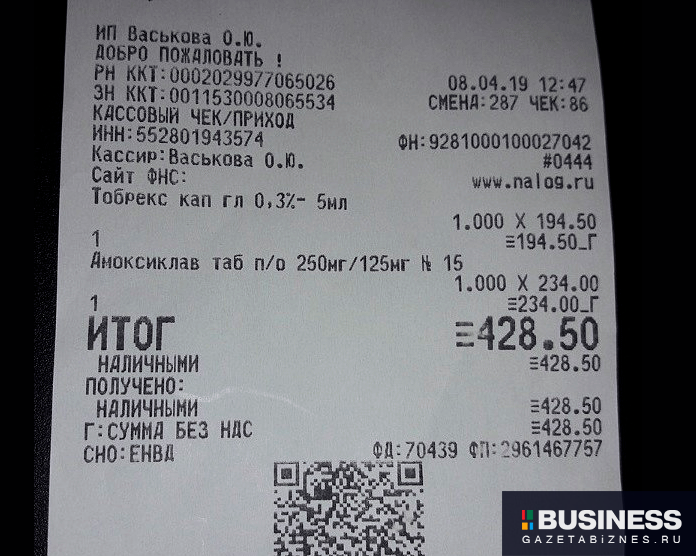
\includegraphics[width=0.75\textwidth]{data/image/check.png}
\caption{Кассовый чек.}
\label{fig:check}
\end{figure}
Перед выполнением OCR-обработки изображение проходит
этап предварительной обработки,
целью которого является повышение качества распознавания текста.
Одной из основных операций является подавление шума
с использованием гауссовой фильтрации.

Пусть исходное изображение задаётся функцией $I : \Omega \rightarrow \mathbb{R}$, где $\Omega$ - множество пикселей изображения.
После применения фильтра формируется сглаженное изображение $I_f = G_\sigma * I$.

Двумерное гауссово ядро определяется следующим выражением
$G_\sigma(x,y)=
\frac{1}{2\pi\sigma^2}
\exp\left(
-\frac{x^2+y^2}{2\sigma^2}
\right).$

Применение гауссовой фильтрации позволяет уменьшить влияние
высокочастотного шума и локальных искажений,
сохранив при этом основные структурные элементы текста.

После этапа сглаживания дополнительно может выполняться
бинаризация изображения.
Например, с использованием порогового преобразования.

Полученное бинарное изображение содержит более контрастные
границы символов,
что повышает точность последующего OCR-распознавания.
После предварительной обработки
алгоритм OCR выделяет текстовые области
и преобразует изображение в последовательность токенов которые далее используются системой анализа транзакций
для извлечения информации о товарах,
стоимости покупок и итоговой сумме чека.
\end{my_example}

Качество OCR-систем обычно оценивается с использованием
метрик Precision и Recall:
\begin{align*}
Precision &= \frac{TP}{TP+FP},
\\
Recall &= \frac{TP}{TP+FN},
\label{eq:metrics}
\end{align*}
где
$TP$ - количество корректно распознанных символов,
$FP$ - количество ложных распознаваний,
$FN$ - количество пропущенных символов.

Дополнительно применяется метрика символьной ошибки (CER):

\begin{equation*}
CER=\frac{S+D+I}{N}.
\label{eq:cer}
\end{equation*}


Для решения задач, связанных с финансовыми транзакциями, широко используются коммерческие и открытые OCR-системы, такие как "Tesseract", "Google Cloud Vision API", "ABBYY FineReader", а также специализированные решения, интегрирующие нейросетевые модели для распознавания текстовой информации на сложных документах. Однако в контексте мультимодальной обработки изображений транзакций универсальные решения остаются ограниченными: большинство систем хорошо справляется с текстом, но не обеспечивает структурированную классификацию транзакций напрямую.

Блок-схема, описывающая принцип работы современной легковесной OCR-системы, включающей в себя интеграцию нейросетевой модели, представлена на рисунке~\ref{fig:easy_ocr}.
\begin{figure}[H]
\centering
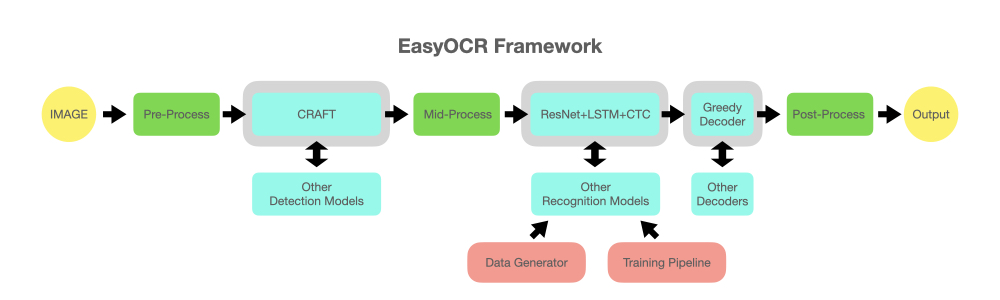
\includegraphics[width=1\textwidth]{data/image/easy_ocr.png}
\caption{Блок-схема EasyOCR.}
\label{fig:easy_ocr}
\end{figure}

Таким образом, можно отсетить, что OCR является необходимым, но недостаточным элементом для создания автоматизированной системы распознавания и классификации транзакций. Эффективное решение требует интеграции OCR с методами извлечения структурированной информации и интеллектуальными алгоритмами классификации.

То, как задается класс дискриминационных вероятностных моделей, используемых для структурированного прогнозирования, описывает формула (\ref{eq:crf}).
\begin{equation}
P(\mathbf{y} \mid \mathbf{x}) =
\frac{1}{Z(\mathbf{x})}
\exp\left(
\sum_{t=1}^{T} \sum_{k} \lambda_k f_k(y_{t-1}, y_t, \mathbf{x}, t)
\right).
\label{eq:crf}
\end{equation}

Байесовская классификация (обычно Наивный байесовский классификатор) — это вероятностный алгоритм машинного обучения, основанный на теореме Байеса. В контексте финансовых транзакций он используется для автоматической категоризации расходов (например, «Продукты», «Кафе», «Такси»), а также для выявления мошенничества. По обыкновению задается формулой (\ref{eq:bc}).

\begin{equation}
P(c \mid \mathbf{x}) =
\frac{P(\mathbf{x} \mid c)\,P(c)}
{\sum_{c' \in \mathcal{C}} P(\mathbf{x} \mid c')\,P(c')}.
\label{eq:bc}
\end{equation}

\section{Извлечение структурированной информации}

Извлечение структурированной информации из изображений финансовых документов является следующим этапом после применения OCR. Оно позволяет преобразовать распознанный текст в структурированные данные, пригодные для анализа и последующей классификации транзакций.

Формально задачу извлечения структурированной информации
можно представить как отображение: $g : T \rightarrow S$, где: $T=\{t_1,t_2,\dots,t_n\}$ - последовательность токенов, $S=\{(k_i,v_i)\}_{i=1}^{m}$ - множество структурированных пар
ключ-значение.

В большинстве случаев, оценка процесса структуризации определается на основе метрик, представленных в таблице~\ref{tab:metrics}.

\begin{tabularx}{\textwidth}{|C|X|}

\caption{Метрики качества извлечения информации.} \label{tab:metrics} \\

\hline
Метрика & Описание \\ \hline
\endfirsthead

\caption{Метрики качества извлечения информации.}\\
\hline
Метрика & Описание \\ \hline
\endhead

Precision &
Показывает, какая доля объектов, предсказанных моделью как положительные, действительно является положительной. 
Высокое значение precision означает низкое количество ложноположительных срабатываний $FP = \displaystyle \frac{TP}{TP+FP}$.  \\ \hline

Recall &
Отражает способность модели находить все положительные объекты.
Высокий recall означает, что модель пропускает мало истинных объектов, то есть количество ложноотрицательных результатов ($FN$) невелико: $\displaystyle \frac{TP}{TP+FN}$.\\ \hline

F1-score &
Гармоническое среднее между precision и recall.
Метрика используется в задачах с несбалансированными классами, когда важно одновременно учитывать и точность, и полноту модели: $\displaystyle 2 \cdot \frac{Precision \cdot Recall}{Precision + Recall}$.\\ \hline

IoU&
Метрика пересечения и объединения двух областей.
Часто применяется в задачах сегментации изображений и object detection для оценки совпадения предсказанной области с истинной разметкой $\displaystyle \frac{A \cap B}{A \cup B}$.\\ \hline

Dice-coef &
Коэффициент сходства между двумя множествами.
Широко используется в медицинской сегментации изображений, так как чувствителен к качеству перекрытия объектов $\displaystyle \frac{2|A \cap B|}{|A|+|B|}$.\\ \hline

Accuracy &
Показывает общую долю правильных предсказаний модели.
Может быть недостаточно информативной для несбалансированных выборок: $\displaystyle \frac{TP+TN}{TP+TN+FP+FN}$.\\ \hline

Specificity &
Характеризует способность модели корректно определять отрицательные объекты.
Высокая specificity означает малое количество ложных тревог: $\displaystyle \frac{TN}{TN+FP}$.\\ \hline

\end{tabularx}

Существующие подходы можно разделить на три основные группы: правило-ориентированные методы, методы машинного обучения и мультимодальные методы. Каждый из подходов имеет свои преимущества и недостатки, отраженные в таблице~\ref{tab:advNdisadv}.

\begin{tabularx}{\textwidth}{|C|X|X|}

\caption{Сравнение подходов к извлечению структурированной информации.} \label{tab:advNdisadv} \\

\hline
Метод &
Преимущества &
Недостатки \\ \hline
\endfirsthead

\caption{Сравнение подходов к извлечению структурированной информации.} \\
\hline
Метод &
Преимущества &
Недостатки \\ \hline
\endhead

Rule-based методы &
Высокая интерпретируемость результатов, простота реализации и низкие требования к вычислительным ресурсам. Позволяют полностью контролировать логику работы системы и легко анализировать причины принятия решений. &
Низкая устойчивость к вариативности входных данных и сложность масштабирования правил. Требуется ручное проектирование и постоянная поддержка набора правил при изменении предметной области. \\ \hline

SVM / Random Forest &
Невысокая вычислительная сложность и хорошая работа на небольших выборках. Методы обладают устойчивостью к переобучению и позволяют эффективно работать со структурированными признаками. &
Необходимость feature engineering и предварительной обработки данных. Качество работы существенно зависит от выбранных признаков и ограничено при обработке сложного контекста. \\ \hline

CNN-based модели &
Эффективное автоматическое извлечение локальных признаков и высокая производительность в задачах компьютерного зрения. Хорошо подходят для обработки изображений и пространственных данных. &
Ограниченный учет глобального контекста и необходимость большого объема размеченных данных. Настройка архитектуры может быть вычислительно затратной и сложной. \\ \hline

RNN / LSTM &
Способность учитывать последовательную структуру данных и работать с временными зависимостями. Подход хорошо подходит для анализа текстов, временных рядов и речевых сигналов. &
Медленное обучение и сложность параллелизации вычислений. Возможны проблемы исчезающего градиента и снижение эффективности при обработке длинных последовательностей. \\ \hline

\end{tabularx}

Правило-ориентированные методы используют заранее заданные шаблоны и регулярные выражения для выделения ключевых полей. Преимуществом является простота реализации и прозрачность работы алгоритма. Однако подход ограничен вариативностью форматов документов: любые изменения шаблона или нестандартные элементы могут привести к ошибкам распознавания.

\begin{my_theorem}
При увеличении вариативности структуры документа
эффективность правило-ориентированных методов
извлечения информации снижается.
\end{my_theorem}

\begin{my_proof}
Правило-ориентированные методы используют фиксированные
шаблоны и регулярные выражения. Пусть множество шаблонов задаётся как $R=\{r_1,r_2,\dots,r_n\}$. Тогда вероятность корректного извлечения поля
определяется согласно формуле (\ref{eq:p_success}).

\begin{equation}
P(success)=
\frac{N_{matched}}{N_{documents}}.
\label{eq:p_success}
\end{equation}

При увеличении числа нестандартных форматов
уменьшается количество совпадений с шаблонами,
что снижает значение $P(success)$.
\end{my_proof}

Классические ML-алгоритмы, такие как случайный лес, SVM или градиентный бустинг, применяются для классификации строк или полей документа после предварительного распознавания текста. Для обучения моделей требуются размеченные наборы данных с указанием позиций и типов полей. Достоинством является возможность адаптации к разным форматам, но качество сильно зависит от размера и качества обучающего корпуса.

Для извлечения сущностей часто используется
задача последовательностной разметки $Y^* = \arg\max_{Y} P(Y|X)$,
где: $X = \{x_1, x_2, \dots, x_n\}$ - входная последовательность, $Y = \{y_1, y_2, \dots, y_n\}$ - последовательность меток.


Современные мультимодальные системы подходы используют сверточные нейронные сети , рекуррентные сети и трансформеры для анализа не только текста, но и визуальной структуры документа. Примеры включают модели, ориентированные на извлечение полей из PDF и изображений чеков. Такие решения способны учитывать расположение текста, таблицы, графические элементы и контекст, что значительно повышает точность извлечения. Недостатком является высокая сложность обучения и необходимость больших размеченных наборов данных.

\begin{my_statement}
Использование визуальных признаков документа
повышает точность извлечения структурированных полей.
\end{my_statement}
\begin{my_proof}
Мультимодальные модели учитывают не только
текстовые токены, но и пространственное расположение элементов.
Пусть итоговое представление документа задаётся как 
$F = \alpha F_t + \beta F_v$, где $F_t$ - текстовые признаки, $F_v$ - визуальные признаки.
Использование пространственных признаков
уменьшает неоднозначность выделения сущностей.
\end{my_proof}

Особое внимание уделяется интеграции OCR с системами извлечения структуры. Даже самые современные OCR-системы предоставляют текстовый поток, который требует дополнительной обработки, чтобы выделить ключевые сущности и превратить их в машинно-структурированные записи транзакций~\cite{babaeva2025}.

Примеры успешного применения таких методов включают автоматизированные системы обработки чеков, квитанций и банковских выписок, используемые в корпоративных финансовых сервисах и аналитических платформах. 

\begin{my_example}
Рассмотрим пример банковской выписки, содержащей табличные данные о финансовых операциях пользователя. 
Документ включает информацию о дате проведения операции, назначении платежа, сумме перевода, а также текущем балансе счета. 
Подобные документы являются типичным примером полуструктурированных данных, где информация представлена одновременно 
в текстовом и табличном формате.

На рисунке~\ref{fig:vipiska} представлен пример шаблона банковской выписки, используемой в качестве входного документа 
для системы анализа и извлечения информации.

\begin{figure}[H]
\centering
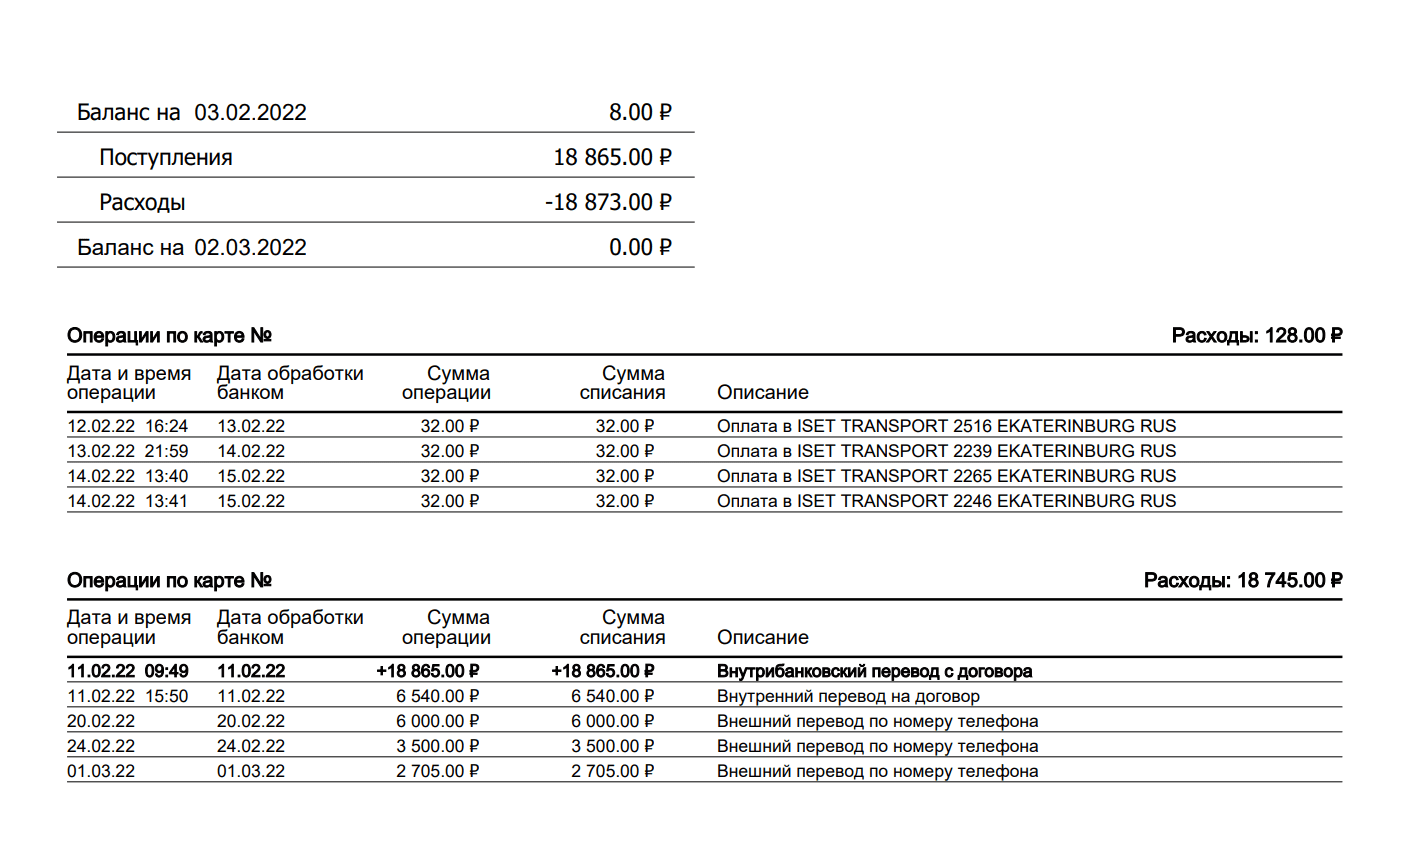
\includegraphics[width=1\textwidth]{data/image/vipiska_template.png}
\caption{Выписка из банка.}
\label{fig:vipiska}
\end{figure}

После процесса OCR-обработки исходное изображение преобразуется в набор текстовых токенов с координатной информацией. 
Каждый токен содержит распознанный текст, а также пространственные признаки, характеризующие его положение на странице документа.
В результате формируется множество токенов $T=\{t_1,t_2,\dots,t_n\}$, где каждый элемент $t_i$ соответствует отдельному текстовому фрагменту документа.
Далее выполняется этап структурирования данных, в рамках которого отдельные токены объединяются в логически связанные сущности. 
После обработки формируются записи следующего вида:
$s_i=(date_i,amount_i,category_i)$
Полученное структурированное представление может использоваться для последующего анализа транзакций, автоматической категоризации расходов, 
выявления аномалий и построения финансовой аналитики.
\end{my_example}

Тем не менее, полностью универсальных решений, способных одновременно обрабатывать различные форматы документов и сразу классифицировать транзакции, в открытой литературе почти не встречается.

Можно сделать промежуточный вывод, что извлечение структурированной информации является ключевым мостиком между распознанным текстом и классификацией транзакций, и именно эта область представляет основной вызов для создания универсальной автоматизированной системы.

Математический метод в статистике и машинном обучении, который разбивает общий логарифм правдоподобия (или общую информацию) модели на отдельные, независимые компоненты, чтобы оценить влияние каждого фактора или взаимодействия между переменными.
\begin{multline*}
\log P(\mathbf{x} \mid \theta) = \log \prod_{t=1}^{T} P(x_t \mid x_{<t}, \theta) = \\
= \sum_{t=1}^{T} \log P(x_t \mid x_{<t}, \theta) = \\
= \sum_{t=1}^{T} \log \frac{\exp(f_\theta(x_{<t}, x_t))}{\sum_{x'} \exp(f_\theta(x_{<t}, x'))}.
\end{multline*}


Математическая функция, используемая в вариационных автокодировщиках для обучения нейросетей. Она выступает в роли «нижней границы» правдоподобия данных, максимизация которой позволяет модели генерировать качественные объекты (например, распознавать текст или сжимать изображения).
\begin{multline*}
\log P(\mathbf{x})
= \log \int P(\mathbf{x}, \mathbf{z})\, d\mathbf{z} = \\
= \log \int \frac{P(\mathbf{x}, \mathbf{z})}{q(\mathbf{z})} q(\mathbf{z})\, d\mathbf{z} \ge \\
\ge \int q(\mathbf{z}) \log \frac{P(\mathbf{x}, \mathbf{z})}{q(\mathbf{z})}\, d\mathbf{z} = \mathcal{L}_{ELBO}.
\end{multline*}

Скрытая марковская модель в контексте OCR — это вероятностный алгоритм, который используется для расшифровки последовательностей, то есть преобразования графических изображений букв в осмысленный текст.
\begin{align*}
P(\mathbf{x}, \mathbf{y}) &= \prod_{t=1}^{T} P(x_t \mid y_t)\, P(y_t \mid y_{t-1}), \\
\hat{\mathbf{y}} &= \arg\max_{\mathbf{y}} P(\mathbf{x}, \mathbf{y}).
\end{align*}

Обучение методом максимального правдоподобия — это процесс подбора параметров математической модели так, чтобы сгенерированные ею данные были максимально похожи на реальные (наблюдаемые) данные. Это базовый принцип обучения многих вероятностных моделей и нейросетей.
\begin{align*}
\theta^* &= \arg\max_{\theta} \sum_{i=1}^{N} \log P(y_i \mid x_i; \theta) = \\
&= \arg\min_{\theta} \sum_{i=1}^{N} -\log P(y_i \mid x_i; \theta).
\end{align*}

Отбор признаков на основе взаимной информации — это метод фильтрации в машинном обучении, который оценивает степень статистической зависимости между каждым признаком и целевой переменной. Он отбирает наиболее информативные признаки, отсекая бесполезные.
\begin{align*}
I(X;Y) &= \sum_{x,y} P(x,y)\log \frac{P(x,y)}{P(x)P(y)}, \\
\mathcal{S}^* &= \arg\max_{\mathcal{S}} I(\mathcal{S}; Y).
\end{align*}

Математический процесс, при котором вычисляется производная логарифма вероятности правильного класса по ненормализованным предсказаниям модели (логитам). Он доказывает, что ошибка для правильного класса представляет собой простую разницу между предсказанием и истиной. Элегантность этого вывода заключается в том, что в результате получается очень простая и интуитивная формула, упрощающая вычисления для алгоритма обратного распространения ошибки. Такой процесс описывается формулой (\ref{eq:logit}).
\begin{equation}
\begin{aligned}
\mathcal{L} &= -\log P(y \mid x) = \\
&= -\log \frac{e^{w_y^\top x}}{\sum_k e^{w_k^\top x}} = \\
&= - w_y^\top x + \log \sum_k e^{w_k^\top x}.
\end{aligned}
\label{eq:logit}
\end{equation}

EM-алгоритм (Expectation-Maximization) для латентного выравнивания в OCR — это математический метод, используемый для распознавания текста. Он применяется для одновременного определения того, где именно в изображении находятся буквы и какие это символы, даже если у системы нет точной посимвольной разметки. Задается формулой (\ref{eq:em}).
\begin{equation}
\begin{aligned}
Q(\theta \mid \theta^{(t)}) &=
\mathbb{E}_{Z \sim P(Z \mid X, \theta^{(t)})}
[\log P(X, Z \mid \theta)], \\
\theta^{(t+1)} &= \arg\max_{\theta} Q(\theta \mid \theta^{(t)}).
\end{aligned}
\label{eq:em}
\end{equation}

Функции потерь — это метрики в машинном обучении, которые измеряют расхождение между истинными и предсказанными распределениями вероятностей. Они оценивают, сколько «информации» или «удивления» теряется при использовании модели.
\begin{gather*}
H(X) = -\sum_x P(x)\log P(x), \\
H(Y \mid X) = -\sum_{x,y} P(x,y)\log P(y \mid x).
\end{gather*}

MAP-вывод (апостериорный максимум) в структурном распознавании текста — это математический метод, который используется для предсказания наиболее вероятного слова или предложения целиком на основе нечеткого изображения, учитывая при этом языковые и пространственные закономерности.
\begin{alignat*}{2}
\hat{\mathbf{y}} &= && \arg\max_{\mathbf{y}} P(\mathbf{y} \mid \mathbf{x}) = \\
&= && \arg\max_{\mathbf{y}} \sum_t \log P(y_t \mid y_{t-1}, x).
\end{alignat*}

Градиент логарифмической функции правдоподобия — это вектор частных производных логарифма функции правдоподобия по всем параметрам модели. В статистике и машинном обучении он показывает направление наибольшего роста правдоподобия и используется для поиска оптимальных параметров.
\begin{alignat*}{2}
\nabla_{\theta} \mathcal{L}
&= && - \sum_i \nabla_{\theta} \log P(y_i \mid x_i; \theta) = \\
&= && \sum_i (P(y \mid x_i) - y_i)x_i.
\end{alignat*}

\section{Классификация транзакций}

Классификация транзакций — это процесс присвоения каждой финансовой операции определённой категории, такой как расход, доход, перевод или оплата услуг. После извлечения структурированной информации из документа, система должна корректно идентифицировать тип транзакции и соответствующие поля, что позволяет интегрировать данные в систему учёта финансов.

Формально задачу классификации транзакций можно представить как отображение $h : S \rightarrow C$, где $S=\{s_1,s_2,\dots,s_n\}$ - множество структурированных записей, $C=\{c_1,c_2,\dots,c_k\}$ - множество категорий транзакций.

Существующие подходы классификации в рамках рассматриваемой предметной области можно разделить на несколько групп:
\begin{itemize}
\item	правило-ориентированные методы,
\item	методы машинного обучения,
\item	глубокое обучение и мультимодальные подходы,
\item	смешанные подходы.
\end{itemize}

Причем в большинстве случаев современные модели классификации определяют категорию транзакции как наиболее вероятный класс
$\hat{c}$. Класс определяется как $\hat{c} =
\arg\max_c P(c|s)
$, где $P(c|s)$ представляет вероятность принадлежности
транзакции $s$ классу $c$.

В таблице~\ref{tab:class_types} отражены современные методы классификации, их преимущества и недостатки.

\begin{tabularx}{\textwidth}{|C|X|X|}

\caption{Сравнение подходов к классификации транзакций.} \label{tab:class_types} \\

\hline
Метод &
Преимущества &
Недостатки \\ \hline
\endfirsthead

\caption{Сравнение подходов к классификации транзакций.} \\
\hline
Метод &
Преимущества &
Недостатки \\ \hline
\endhead

Rule-based подход &
Высокая интерпретируемость результатов и возможность полного контроля логики классификации. 
Подход прост в реализации, не требует большого объема обучающих данных и обеспечивает стабильную работу на заранее определённых сценариях обработки транзакций. &
Низкая гибкость и слабая адаптация к изменяющимся данным. 
При увеличении числа категорий транзакций существенно возрастает сложность поддержки правил, а также ухудшается устойчивость к вариативности текстовых описаний операций. \\ \hline

SVM &
Хорошая обобщающая способность и эффективность работы на небольших наборах данных. 
Метод обеспечивает устойчивость к переобучению и позволяет получать качественные результаты при использовании информативных признаков. &
Требует feature engineering и предварительного извлечения признаков. 
Качество классификации сильно зависит от этапа подготовки данных, а обработка сложного контекста и длинных текстов ограничена. \\ \hline

TF-based модели &
Высокая точность классификации и способность учитывать контекст всей последовательности текста. 
Модели данного типа эффективно работают с неструктурированными описаниями транзакций и поддерживают transfer learning на предобученных языковых моделях. &
Высокая вычислительная сложность и значительные требования к аппаратным ресурсам. 
Для обучения и инференса необходимы GPU-ускорители, а также большие объемы размеченных данных. \\ \hline

Hybrid подход &
Комбинация преимуществ нескольких методов позволяет повысить устойчивость и качество классификации. 
Гибридные архитектуры могут совмещать интерпретируемость rule-based систем и точность нейросетевых моделей. &
Сложность интеграции и увеличенные затраты на разработку и сопровождение системы. 
Настройка взаимодействия между компонентами требует дополнительной оптимизации и усложняет архитектуру решения. \\ \hline

\end{tabularx}

В целом, несмотря на существование множества алгоритмов классификации~\cite{poladov2024}, практически не встречаются решения, объединяющие распознавание текста, извлечение структуры и автоматическую классификацию транзакций в одном универсальном конвейере, что подчеркивает актуальность дальнейших исследований и разработки нового подхода.

В последние годы в научных исследованиях и индустриальных разработках активно рассматриваются мультимодальные подходы, направленные на одновременную обработку визуальной и текстовой информации. Такие решения предполагают использование единых моделей, которые принимают на вход изображение документа и формируют итоговое представление данных без явного разделения на этапы OCR, структуризации и классификации.

\begin{my_example}
Рассмотрим процесс обработки текстового описания банковской транзакции с использованием трансформерной архитектуры. 
На первом этапе исходный текст проходит процедуру токенизации, в рамках которой строка разбивается на последовательность отдельных токенов, 
соответствующих словам, подсловам или специальным символам.
Например, описание транзакции \texttt{"PAYMENT TO AMAZON STORE"} может быть преобразовано в последовательность токенов $\{t_1,t_2,t_3,t_4\}$.

Далее каждый токен отображается в векторное пространство фиксированной размерности с помощью embedding-представления. 
В результате формируется последовательность dense-векторов.

\begin{equation*}
X=\{x_1,x_2,\dots,x_n\},
\quad
x_i \in \mathbb{R}^d,
\end{equation*}
где $n$ - количество токенов во входной последовательности, $d$ - размерность embedding-пространства, $x_i$ - векторное представление токена $t_i$.

Embedding-векторы позволяют преобразовать текстовую информацию в числовую форму, пригодную для обработки нейронной сетью. 
При этом семантически близкие слова получают близкие представления в пространстве признаков.

На рисунке~\ref{fig:transformer_pipeline} представлена общая схема обработки транзакции трансформерной моделью.

\begin{wrapfigure}{r}{0.5\textwidth}
\centering
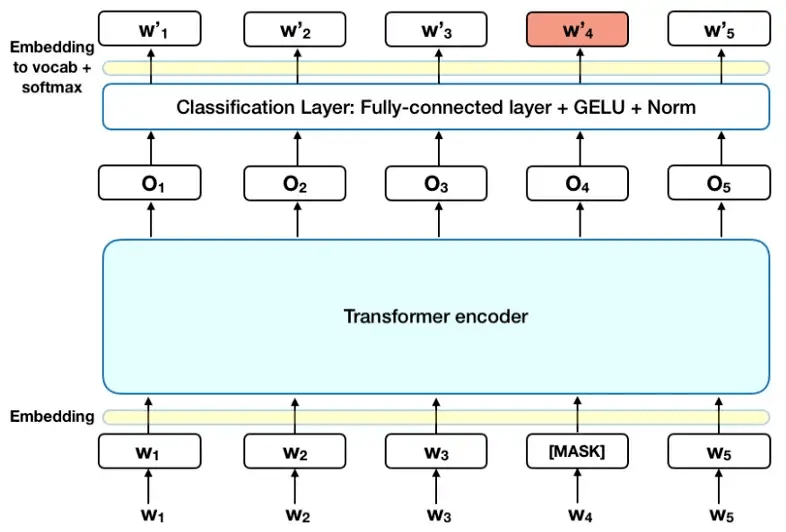
\includegraphics[width=0.5\textwidth]{data/image/bert_model.png}
\caption{Схема трансформера.}
\label{fig:transformer_pipeline}
\end{wrapfigure}


После формирования embedding-представлений последовательность подается в трансформерную модель, 
где механизм self-attention вычисляет зависимости между всеми токенами входной последовательности. $P(y=k \mid \mathbf{x}) =
\frac{\exp(\mathbf{w}_k^\top \mathbf{x})}
{\sum_{j=1}^{K} \exp(\mathbf{w}_j^\top \mathbf{x})}$. Это позволяет модели учитывать глобальный контекст описания транзакции и эффективно выявлять семантические связи между словами.

Полученное контекстное представление используется на этапе классификации для определения категории транзакции, 
например: покупки, переводы, коммунальные платежи или подписки.

\end{my_example}

В основе подобных подходов лежат глубокие нейронные сети, комбинирующие методы компьютерного зрения и обработки естественного языка~\cite{jin2025}. $\mathcal{L} =
- \sum_{k=1}^{K} y_k \log P(y=k \mid \mathbf{x})$. Как правило, используются сверточные нейронные сети для извлечения визуальных признаков и трансформерные архитектуры для работы с текстом и контекстом документа. Примерами таких моделей являются универсальные документоориентированные модели, способные выполнять несколько задач одновременно.

Несмотря на концептуальную привлекательность таких подходов, их практическое применение в задачах анализа финансовых транзакций сопровождается рядом существенных ограничений. Во-первых, такие модели обладают высокой архитектурной сложностью и требуют значительных вычислительных ресурсов как на этапе обучения, так и при эксплуатации. Во-вторых, обучение подобных систем требует больших объёмов размеченных данных, что особенно проблематично в финансовой сфере из-за конфиденциальности и разнообразия форматов документов~\cite{masri2024}. 

$P(\mathbf{x}, \mathbf{y}) = \prod_{t=1}^{T} P(x_t \mid y_t)\, P(y_t \mid y_{t-1})$. Отдельной проблемой является низкая интерпретируемость мультимо-дальных моделей. $\mathcal{L} =
\mathcal{L}_{data} + \lambda \|\theta\|_2^2$. В случае интеграции таких решений в системы учёта личных или корпоративных финансов модель фактически становится «чёрным ящиком»: сложно определить, на основании каких признаков была выполнена классификация транзакции или допущена ошибка. Это существенно осложняет отладку системы, её масштабирование и использование в задачах, где требуется высокая прозрачность принятия решений.

\begin{my_theorem}
Увеличение архитектурной сложности модели
снижает интерпретируемость процесса
классификации транзакций.
\end{my_theorem}
\begin{my_proof}
Рассмотрим нейронную сеть глубины $L$, задающую отображение
из пространства признаков входной транзакции $x \in \mathbb{R}^d$
в пространство предсказаний $y$:
$f(x) = h_L, \quad
h_l = \sigma(W_l h_{l-1} + b_l), \quad l = 1,\dots,L.
$

Функция $f(x)$ представляет собой композицию нелинейных преобразований:
$
f(x) = f_L \circ f_{L-1} \circ \dots \circ f_1(x).
$

При увеличении числа слоёв возрастает степень нелинейности отображения,
что приводит к усложнению декомпозиции итогового решения
по входным признакам.

Рассмотрим вклад отдельного признака $x_i$ в предсказание модели.
Формально чувствительность выхода можно смело выразить через градиент
$
S_i = \frac{\partial f(x)}{\partial x_i}.
$

В глубокой модели этот градиент раскрывается по правилу цепочки
$
\frac{\partial f}{\partial x}
=
\prod_{l=1}^{L}
\frac{\partial h_l}{\partial h_{l-1}}
=
\prod_{l=1}^{L}
J_l.
$

При увеличении $L$ произведение якобианов становится
либо сильно сглаженным, либо нестабильным,
что затрудняет интерпретацию влияния отдельных признаков.

Дополнительно, пространство скрытых представлений $h_l$
становится всё более абстрактным $h_l \in \mathbb{R}^{d_l}, \quad d_l \uparrow \text{или фиксировано}$ и семантическое соответствие между компонентами $h_l$
и исходными признаками $x_i$ теряется.

Таким образом, увеличение глубины и числа параметров модели
приводит к росту выразительной мощности,
но снижает интерпретируемость предсказаний
за счёт усложнения функциональной декомпозиции и ослабления связи
между входными признаками и выходом модели.
\end{my_proof}

Кроме того, существующие мультимодальные решения, как правило, раз-рабатываются как универсальные модели общего назначения и плохо адаптируются под специфические требования конкретных финансовых систем. Их интеграция в уже существующие приложения часто ограничена закрытой архитектурой, отсутствием гибкой настройки и зависимостью от внешних сервисов.

\begin{my_statement}
Модульная архитектура системы упрощает
анализ ошибок и масштабирование
процесса классификации транзакций.
\end{my_statement}
\begin{my_proof}
Разделение системы на независимые этапы
OCR, извлечения структуры и классификации
позволяет верно локализовать ошибки.
Пусть общий конвейер определяется как
$Pipeline=O \circ E \circ C$
где:
$O$ - OCR,
$E$ - извлечение структуры,
$C$ - классификация.
Независимость этапов позволяет
оптимизировать компоненты отдельно, а также отлаживать процесс на каждом из этапов.
\end{my_proof}

Таким образом, несмотря на активное развитие современных комбини-руемых подходов, в настоящий момент они не представляют собой универсального и практического решения для автоматизированного распознавания и классификации финансовых транзакций. Это обосновывает целесообразность разработки модульного, интерпретируемого конвейера, в котором этапы распознавания, структуризации и классификации могут быть независимо анализируемы, улучшены и интегрированы в системы учёта финансов.

В таблице~\ref{tab:1234} представлены данные из csv-файла.

\begin{tabularx}{\textwidth}{|X|X|X|X|}

\caption{Таблица из csv-файла.}
\label{tab:1234} \\

\hline
Этап &
Среднекв. величина &
Относительная ошибка &
Абсолютная ошибка 
\\ \hline
\endfirsthead

\caption{Таблица из csv-файла.} \\
\hline
Этап &
Среднекв. величина &
Относительная ошибка &
Абсолютная ошибка 
\\ \hline
\endhead

\csvreader[
separator=comma,
late after line=\\\hline
]
{data/table/1dfixedsrc.csv}
{}
{%
\csvcoli &
\csvcolii &
\csvcoliii &
\csvcoliv}

\end{tabularx}


\section{Ключевые выводы}

Проведённый обзор существующих методов и решений в области анализа финансовых документов на основе изображений показывает, что, несмотря на значительный прогресс в технологиях компьютерного зрения и обработки естественного языка~\cite{krasochkin2025}, задача автоматизированного распознавания и классификации транзакций остаётся нерешённой в комплексном виде.

Большинство существующих подходов ориентированы на решение отдельных подзадач. OCR-системы демонстрируют высокую точность при извлечении текстовой информации, однако не обеспечивают корректную интерпретацию и семантическую классификацию транзакций. Методы структурного анализа позволяют выделять отдельные элементы документа, такие как суммы, даты и наименования, но, как правило, требуют ручной настройки под конкретные форматы и плохо масштабируются на разнообразные источники данных. Алгоритмы классификации транзакций, в свою очередь, предполагают наличие уже структурированных входных данных и не предназначены для работы напрямую с изображениями, мультимодальные решения, объединяющие несколько этапов обработки, теоретически способны устранить данные ограничения, однако на практике обладают рядом существенных недостатков

Дополнительным фактором, усложняющим решение задачи, является отсутствие единых стандартов представления финансовых документов. Форматы чеков, выписок и платёжных подтверждений существенно различаются в зависимости от банка, платёжного сервиса и страны, что снижает эффективность специализированных и жёстко настроенных алгоритмов.

Таким образом, анализ существующих решений позволяет сформулировать ключевую научно-практическую проблему: отсутствие универсальной, интерпретируемой и масштабируемой системы, способной выполнять распознавание, структуризацию и классификацию финансовых транзакций на основе изображений различных типов документов.




% 5. Заключение
\structsection{Заключение}

В ходе прохождения учебной практики (научно-исследовательской работы) были выполнены начальные этапы исследования в рамках темы магистерской диссертации, посвящённой автоматизированному распознаванию и классификации транзакций на основе анализа изображений.

В рамках работы была сформулирована и обоснована актуальность выбранной темы, связанная с ростом объёмов финансовых данных, представленных в визуальной форме, а также с ограничениями существующих систем автоматизированного учёта личных финансов. Проведён анализ предметной области, включающий изучение структуры финансовых документов и особенностей их представления в виде изображений различного типа.

Был выполнен обзор и систематизация существующих подходов к решению задачи, включая методы оптического распознавания текста, алгоритмы извлечения структуры документов, методы классификации транзакций, а также мультимодальные решения. Проведённый анализ позволил выявить достоинства и недостатки указанных подходов, а также определить ключевые ограничения, препятствующие созданию универсальных систем анализа транзакционных документов.

По результатам исследования сделан вывод о целесообразности применения модульного подхода к построению автоматизированной системы, включающего отдельные этапы распознавания, структуризации и классификации данных. Такой подход обеспечивает гибкость, масштабируемость и возможность интеграции разрабатываемых решений в прикладные системы учёта финансов. Схема такого решения продемонстрирована на рисунке~\ref{fig:pipeline}.

\begin{figure}[H]
\centering
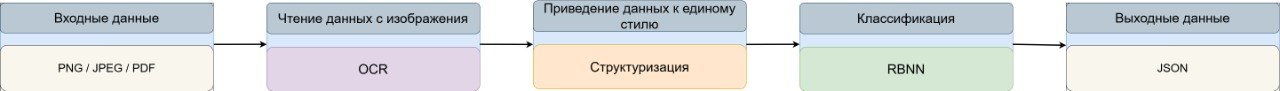
\includegraphics[width=1\textwidth]{data/image/pipeline.png}
\caption{Блок-схема системы.}
\label{fig:pipeline}
\end{figure}

Полученные в ходе практики результаты и сформированные выводы послужат основой для дальнейшей научно-исследовательской работы, направленной на разработку и экспериментальное исследование алгоритмов автоматизированного анализа финансовых документов в рамках магистерской диссертации.

За время практики были реализованы следующие компетенции, описанные в таблице~\ref{tab:competencies}:

\begin{tabularx}{\textwidth}{|C|X|X|}

\caption{Реализованные компетенции.} \label{tab:competencies} \\

\hline
Шифр компетенции & Расшифровка приобретаемой компетенции & Расшифровка освоения компетенции \\ \hline
\endfirsthead

\caption{Реализованные компетенции.} \\
\hline
Шифр компетенции & Расшифровка приобретаемой компетенции & Расшифровка освоения компетенции \\ \hline
\endhead

УК-1 & Способен осуществлять критический анализ проблемных ситуаций на основе системного подхода, вырабатывать стратегию действий & Проведён анализ предметной области автоматизированной обработки финансовых документов, выявлены ограничения существующих подходов и сформулирована стратегия дальнейшего исследования \\ \hline

УК-4 & Способен применять современные коммуникативные технологии, в том числе на иностранном(ых) языке(ах), для академического и профессионального взаимодействия & Выполнен поиск и изучение научных публикаций на русском и английском языках, подготовлены материалы доклада и презентации по теме исследования \\ \hline

УК-6 & Способен определять и реализовывать приоритеты собственной деятельности и способы ее совершенствования на основе самооценки & Самостоятельно сформирована и уточнена тема исследования, спланированы этапы научно-исследовательской работы и определены направления дальнейшего развития \\ \hline

ОПК-1 & Способен находить, формулировать и решать актуальные проблемы прикладной математики, фундаментальной информатики и информационных технологий & Сформулирована актуальная задача автоматизированного распознавания и классификации транзакций на основе анализа изображений и определены основные направления её решения \\ \hline

ОПК-2 & Способен применять компьютерные/суперкомпьютерные методы, современное программное обеспечение (в том числе отечественного производства) для решения задач профессиональной деятельности & Изучены и проанализированы современные OCR-системы, методы компьютерного зрения и модели машинного обучения, применяемые для анализа документов \\ \hline

ОПК-3 & Способен проводить анализ математических моделей, создавать инновационные методы решения прикладных задач профессиональной деятельности в области информатики и математического моделирования & Проведён сравнительный анализ существующих моделей и подходов, определены их достоинства и недостатки, сформулированы требования к разрабатываемому модульному конвейеру \\ \hline

\end{tabularx}


% 6. Литература
\structsection{Список использованной литературы}

\printbibliography[heading=none]

% 7. Приложение
\appendix
\structsection{Приложение}
\begin{lstlisting}
import cv2
from sklearn.model_selection import train_test_split
from src.plugins.classification.custom_rule_based import RuleClassifier
from src.plugins.classification.ml import MLClassifier
from src.plugins.ocr.easy import EasyOCRWrapper
from src.plugins.ocr.rapid import RapidOCRWrapper
from src.plugins.structurer.temp import SimpleStructurer
from src.plugins.pipeline.pipeline import Pipeline
from src.utils.data_load import load_dataset
from src.utils.image_processor import Preprocessor


def run_experiment():
    # 1. обучаем  ML
    texts, labels = load_dataset("data/new_dataset.csv")

    X_train, X_test, y_train, y_test = train_test_split(
        texts, labels, test_size=0.3, random_state=42
    )

    ml = MLClassifier()
    ml.train(X_train, y_train)

    structurer = SimpleStructurer()
    preprocessor = Preprocessor()

    # 2. OCR модели
    ocr_models = {
        "Rapid": RapidOCRWrapper(),
        "EasyOCR": EasyOCRWrapper(),
    }

    # 3. test изображения
    test_images = []

    for type_ in ['food', 'transport', 'shopping']:
        for j in range(1,6):
            test_images.append((f"data/{type_}_sample/{type_}_{j}.jpg", f"{type_}"))

    print(test_images)

    results = {
        "RAW": {},
        "PREPROCESSING": {}
    }

    for mode in ["RAW", "PREPROCESSING"]:
        print(f"\n\n===== MODE: {mode} =====")

        for ocr_name, ocr in ocr_models.items():
            correct = 0

            print(f"\n=== {ocr_name} ({mode}) ===")

            for path, true_label in test_images:
                image = cv2.imread(path)

                if mode == "PREPROCESSING":
                    image = preprocessor.process(image)

                text = ocr.extract_text(image)
                doc = structurer.structure(text)
                pred = ml.classify(doc)

                print(f"\nImage: {path}")
                print(f"Predicted: {pred} | True: {true_label}")

                if pred == true_label:
                    correct += 1

            acc = correct / len(test_images)

            if ocr_name not in results[mode]:
                results[mode][ocr_name] = acc

            print(f"\n{ocr_name} {mode} accuracy: {acc}")

    return results


def main():
    # 1. Загружаем ds
    texts, labels = load_dataset("data/new_dataset.csv")

    X_train, X_test, y_train, y_test = train_test_split(
        texts, labels, test_size=0.3, random_state=42
    )

    # 2. Обучаем ML классификатор
    ml_classifier = MLClassifier()
    ml_classifier.train(X_train, y_train)

    structurer = SimpleStructurer()
    preds = []

    for text in X_test:
        document = structurer.structure(text)  # важно!
        pred = ml_classifier.classify(document)
        preds.append(pred)

    accuracy = sum([1 for p, t in zip(preds, y_test) if p == t]) / len(y_test)

    print("ML accuracy:", accuracy)

    # 3. init компонентов
    ocr = EasyOCRWrapper()
    structurer = SimpleStructurer()
    rule_classifier = RuleClassifier()

    # 4. Создаем pipeline 
    pipeline_rule = Pipeline(ocr, structurer, rule_classifier)
    pipeline_ml = Pipeline(ocr, structurer, ml_classifier)

    # 5. test изображение
    image = cv2.imread("data/food_sample/food_1.jpg")

    result_rule = pipeline_rule.run(image)
    result_ml = pipeline_ml.run(image)

    print("=== Rule-based ===")
    print(result_rule)

    print("\n=== ML ===")
    print(result_ml)


if __name__ == "__main__":
    main()
    results = run_experiment()
    print("\n=== FINAL RESULTS ===")
    for mode, res in results.items():
        print(f"\n--- {mode} ---")
        for k, v in res.items():
            print(f"{k}: {v}")
\end{lstlisting}



\end{document}